% LaTeX Template
% \documentclass[autodetect-engine,dvipdfmx-if-dvi,ja=standard]{bxjsarticle}
\documentclass[a4j,10ptj,fleqn]{ltjsarticle}  % LuaLaTeX
% \documentclass[uplatex,a4j,twoside,fleqn]{jsarticle}  % upLaTeX

  \usepackage{ifluatex}
  \ifluatex
    \usepackage{graphicx}
    \usepackage{luatexja-otf}
    % \usepackage[ms]{luatexja-preset}
    \usepackage[intlimits]{amsmath}
    \usepackage{amssymb}
    % \usepackage{unicode-math}
    % \setmainfont[Ligatures=TeX]{Times New Roman}
    % \setmonofont[Ligatures=TeX]{Inconsolatazi4}
    % \unimathsetup{math-style=ISO,bold-style=ISO}
    % \usepackage{textgreek}  % 立字alpha
    \usepackage{upgreek}  % 立字mu
  \else
    \usepackage[dvipdfmx]{graphicx,color}
    \usepackage{amsmath}  % \allowdisplaybreaks, align, flagin
    %\usepackage{amssymb}  % 特殊記号用 (txfontsを使う場合は不要)
    \usepackage{inconsolata}
    \usepackage{txfonts}  % TXフォント (Times Roman系フォント)
  \fi
  \usepackage{mathrsfs}	 % \mathscr用
%   \usepackage{siunitx}  % SI単位系
  \usepackage{booktabs}  % 綺麗な表組みのためのパッケージ
  \usepackage{multirow}  % 複数行や複数列にまたがる表組み
  \usepackage{type1cm}  % フォント拡大縮小
  \usepackage{scalefnt}	 % フォント拡大縮小
  \usepackage{comment}  % 複数行のコメントアウト
  \usepackage{subfigure}  % 図を複数並べる

  \usepackage[nocolsep]{dotseqn}  % 数式を点線で結ぶ
  \makeatletter
  \renewcommand\EqnDots{\leaders\hbox{\kern1\p@ .\kern1\p@}\hfill}
  \makeatother
  \renewcommand{\textbf}[1]{{\bfseries\sffamily#1}}  %太字にする際ゴシック体とセリフ体とを区別なく太くする

  \usepackage{jsbook2thesisL}

  % citation
  \usepackage{overcite}
  \renewcommand\citeform[1]{(#1)}

  % Use \mathrm \boldsymbol
  \ifluatex
    \def\boldsymbol#1{{\symbf{#1}}}
    %\def\mathrm#1{{\symup{#1}}}
    %\newcommand{\alphaup}{\symup{\alpha}}
    %\newcommand{\muup}{\symup{\mu}}
    \newcommand{\alphaup}{\mbox{\textalpha}}
    \newcommand{\muup}{\upmu}
    \newcommand{\thetaup}{\mbox{\straighttheta}}
    \newcommand{\vol}{\mbox{\usefont{T1}{ptm}{m}{it}{v}}}
  \else
    \def\boldsymbol#1{%
      \def\moji{#1}% 
      \def\temp{v}% 
      \ifx\moji\temp%vだけフォント変更(使用時は個別に{}で囲む必要あり)
        {\mbox{\usefont{T1}{cmr}{bx}{it} {#1}}}%
      \else%
        {\mbox{\boldmath ${#1}$}}%
      \fi}
  \fi

  \usepackage{lipsum}  % ダミーテキスト用

% 文書
\begin{document}
  \pagenumbering{arabic}

% タイトル
\begin{center}
{\scalefont{2}計画書}
\end{center}
\vspace{0.3cm}
\begin{flushright}
{20XX年XX月XX日作成}
\\
{〇〇 〇〇}
\end{flushright}

% 本文
\section{研究題目}
〇〇〇〇〇〇〇〇

\section{研究背景}
Burgersベクトルは,現配置において式\eqref{eq_bergers_vector}で表される~\cite{kondo1955non-riemannian}.
%
\begin{equation}
  \label{eq_bergers_vector}
    \tilde{B}{}^{a}
    = -\int_{\mathscr{S}} \left[ \hat{T}{}^{..a}_{bc} + \frac{1}{2} C^{\ell{}-1ae}
      \left( \hat{R}{}_{bc[de]} + \hat{R}{}_{bc(de)} \right) x^{d} \right] \mathrm{d} x^{b} \wedge \mathrm{d} x^{c}
  \dotfill
\end{equation}
%
これを図示すると,図\ref{fig_paper_irasutoya}のようになる.
%
\begin{figure}[bp]
    \centering
    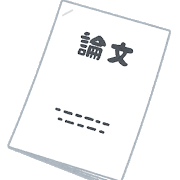
\includegraphics{./figure/document_ronbun_taba.png}
    \caption{Paper.}
    \label{fig_paper_irasutoya}
\end{figure}
%

% 参考文献
\bibliographystyle{./chap/sjunsrt_d.bst}
\bibliography{./chap/reference.bib}

\end{document}
